\documentclass[11pt, a4paper]{scrartcl}

\usepackage[left=3cm, right=3cm, top=3cm, bottom=3cm]{geometry}
\usepackage{graphicx}
\usepackage{array}
\usepackage{amsmath}


\newcommand{\git}{\mathbin{
  \mathchoice{/\mkern-6mu/}% \displaystyle
    {/\mkern-6mu/}% \textstyle
    {/\mkern-5mu/}% \scriptstyle
    {/\mkern-5mu/}}}% \scriptscriptstyle


\title{Monte Carlo Methods - Sheet 4}
\subtitle{Ising Model: Wolff algorithm}
\author{Tobias Sizmann}

\begin{document}
\maketitle
\textit{"Nonlocal" truely is a scary word for every physics student. What follows is usually a mess of summation and integration over variables and their primed counterparts. It is so scary that even one of the most gifted physicists - Albert Einstein - labeled it as "spooky". This is completely taken out of context and has nothing to do with what follows except for the word "nonlocal". But it produces an interesting anecdote - which is obviously the only purpose of this text.}
\section{Introduction}
    We have seen that the Metropolis algorithm suffers from a bad disease: Critical slowing down. This is intrinsic to all local algorithms due to the low probability of a single spin flip. The obvious solution is a nonlocal (\textit{scaaaary}) algorithm. And so the german physicist Ulli Wolff proposed the Wolff algorithm in 1989. Instead of flipping a single spin the algorithm builds a cluster and then flips the whole cluster at once. If the cluster mechanism is constructed properly, it satisfies detailed balance and the algorithm samples the desired probability distribution.
\section{The Wolff algorithm}
    In the special case of the Ising model the Wolff algorithm is defined by the following steps
    \begin{enumerate}
        \item Choose an initial spin site randomly. This is the first site of the cluster. It has spin $s_{initial}$.
        \item Whenever a spin is added to the cluster, consider all neighbors that have spin $s_{neighbor} = s_{initial}$ and are not yet part of the cluster. Add each of those neighbors to the cluster with a probability $P_{add} = 1 - \exp(-2 \beta J)$
    \end{enumerate}
    In terms of implementation the algorithm suggests the use of a ``first in first out'' data structure like a queue. It can be shown that this algorithm satisfies detailed balance. Note that the time complexity for one cluster flip at maximum is in the order of one Metropolis sweep. In the introduction the claim has been made, that this algorithm is advantageous at the critical point. This can be seen immediately now: The probability to add an adjacent spin with same orientation to the cluster in the case of the Ising model at the critical point is $P_{add} = 1 - \exp(-2 \beta_c J) = 0.59$ which is rather large considering that for each added spin several new spins are considered (at least at the beginning of the cluster growth). Here an assumption has been made, however, namely that the density of adjacent spins with the same orientation is high. This is given physically: The spatial correlation length diverges at the critical point. We therefore expect the average cluster size $\langle n \rangle$ at the critical point to be way larger than 1 consequently reducing autocorrelation.
\section{Comparion: Wolff vs Metropolis}
    Goal of this section is to compare results of Wolff and Metropolis sample generation. Note that in terms of time complexity a Metropolis sweep always cost more or the same as a Wolff cluster flip. Therefore if the errors on estimates are lower for the Wolff algorithm than for Metropolis algorithm if the same amount of sweeps and cluster flips has been done, the Wolff algorithm proofs its superiority for this specific case of external parameters (here: temperature, lattice extend, coupling, external magnetic field). Be careful, as this argument does not work the other way around.

    All following discussions are done on a 64x64 grid with $J = 1$ and $B_{ext} = 0$ with 10000 thermalized sweeps/clusterflips. Metropolis samples from $T = 1$ to $T = 4$ with stepsize $\Delta T = 0.1$ have been generated. For the region $T = 2.1$ to $T = 2.4$ both Metropolis and Wolff samples have been generated with a stepsize of $\Delta T = 0.02$. The results are depicted in figure 1 (Metropolis) and figure 2 (Metropolis and Wolff in the critical region). Comparison of the data concludes that the errors are smaller for the Wolff samples around the critical point at $T_c = 2.28 \pm 0.02$ (estimated by the peaks of the susceptibilities from the plots) and therefore the Wolff algorithm has been determined to be more efficient around the critical point compared to the Metropolis algorithm (i.e. more independent configurations are being generated in the same time).

    \begin{figure}
    \begin{centering}
        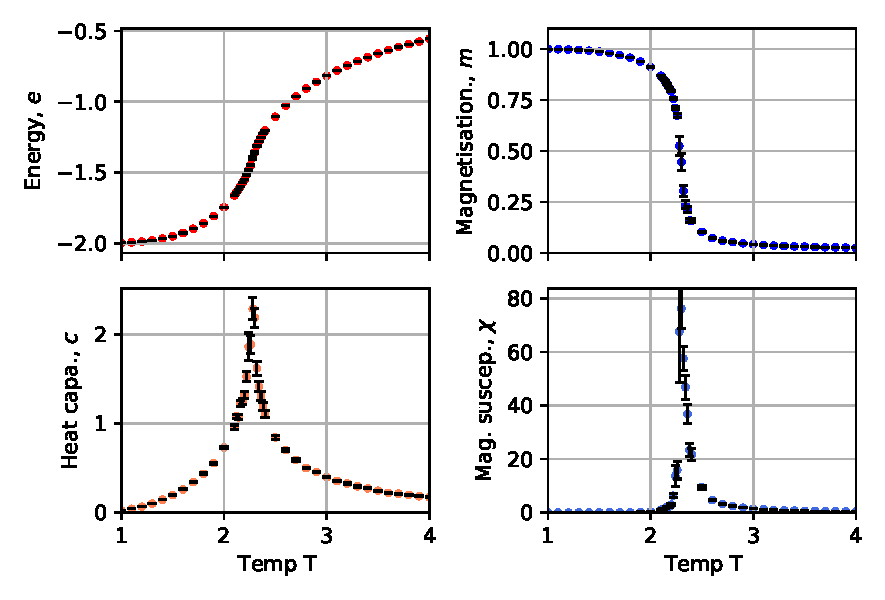
\includegraphics{obs_metro.pdf}
        \label{obs_metro}
        \caption{\textbf{Metropolis algorithm: } Results of 10000 thermalized Metropolis sweeps.}
    \end{centering}
    \end{figure}

    \begin{figure}
    \begin{centering}
        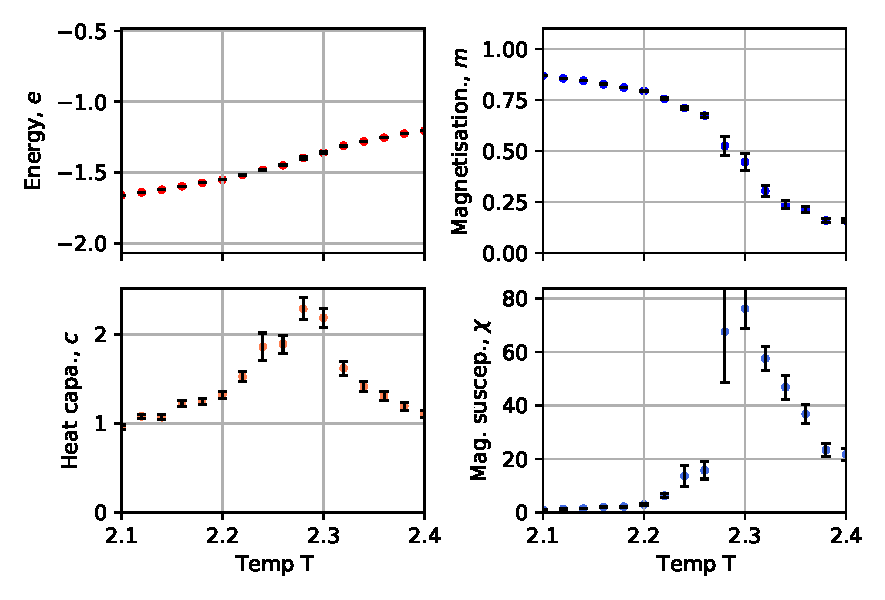
\includegraphics{obs_metro_critical.pdf}
        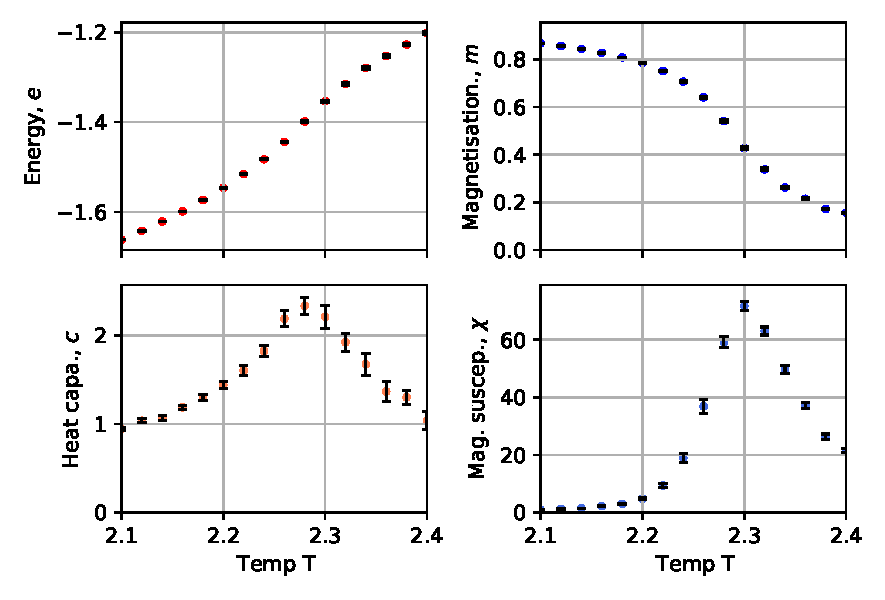
\includegraphics{obs_wolff_critical.pdf}
        \label{obs_critical}
        \caption{\textbf{Critical region: } Results of 10000 thermalized Metropolis sweeps (upper half) and 10000 thermalized Wolff clusterflips (lower half) in the critical region. Just by eye one can already see that the errors are reduced for the Wolff algorithm.}
    \end{centering}
    \end{figure}

\section{Clustersize as function of temperature}
    \begin{figure}
    \begin{centering}
        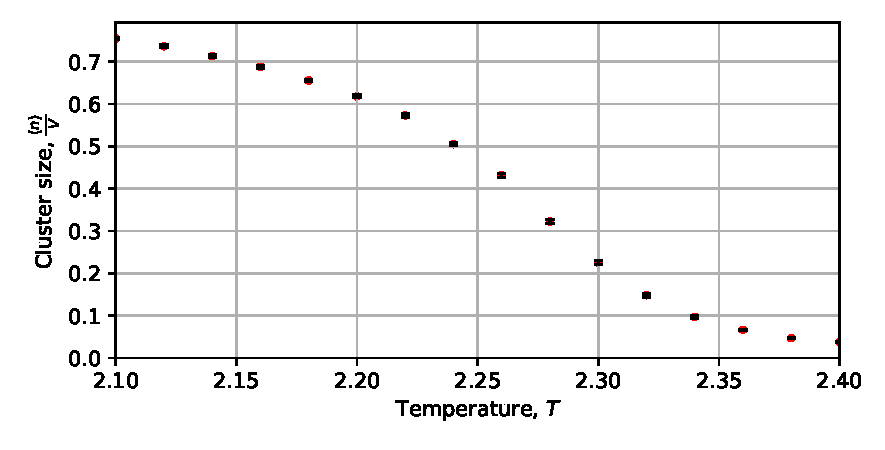
\includegraphics{clusters.pdf}
        \caption{\textbf{Clustersize as function of temperature: } For each datapoint a sample of 10000 thermalized cluster flips has been generated and the average cluster size has been plotted. }
    \end{centering}
    \end{figure}

    For the same Wolff samples as in last section the average cluster size has been plotted in fig. 3. In the low temperature limit the algorithm flips almost the whole lattice every step. This is expected as the acceptance pobability is converging towards 1. In the high temperature limit the opposite is the case. The Wolff algorithm becomes almost a single flip algorithm because the acceptance probability is converging towards 0.

\section{Autocorrelation: Wolff vs. Metropolis}
    Low autocorrelation times are critical for the efficiency of an algorithm. In the following the autocorrelation times for Wolff and Metropolis samples around the critical point are compared. It should be noted that the Markov time units from Wolff and Metropolis can not be directly compared. What we want to know is how many independent samples can be generated with given computer time. This calculation is flawed from the beginning as the computer time depends on exterior parameters like the computer architecture. Maybe the Wolff algorithm is more efficient on a single core machine but the Metropolis algorithm can be parallelized more easily (just one consideration of many). Due to these complications one uses the rough estimate that $\tau_{int, Metropolis} = \frac{\langle n \rangle}{V} \tau_{int, Wolff}$. The results are depicted in fig. 4. As one can see, the Wolff algorithm outperforms the Metropolis algorithm up to a factor of $\approx 1000$ in the critical region.
    \begin{figure}
    \begin{centering}
        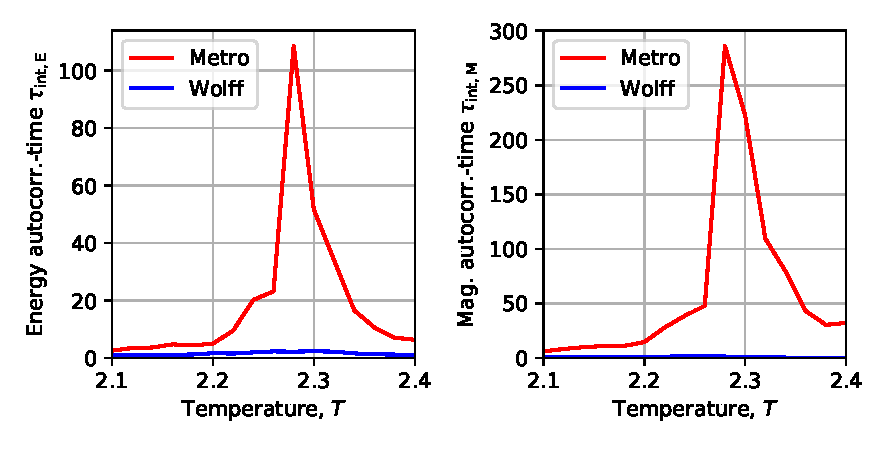
\includegraphics{autocorrelations.pdf}
        \caption{\textbf{Autocorrelations of Metropolis and Wolff: } Plotted are the autocorrelation times for energy (left) and magnetisation (right) for the Wolff (blue) and Metropolis (red) samples from section 3. The autocorrelation times are plotted in units of Metropolis sweeps, i.e., the autocorrelation times from Wolff samples in Wolff Markov time are multiplied by $\frac{\langle n \rangle}{V}$}
    \end{centering}
    \end{figure}

\end{document}
